% !TeX root = RJwrapper.tex
\title{The reproductive and parental care transcriptome of the rock dove}
\author{by Suzanne H. Austin \footnote{equal contribtion, currently at the
  University of Oregon}, Rayna M Harris \footnote{equal contribtion}, Andrew S. Lang, Victoria S. Farrar, April Booth, Tanner Feustel, Matthew D. MacManes, Rebecca M. Calisi \footnote{corresponding author}}

\maketitle

\abstract{%
In animals that exhibit a parental care reproductive strategy,
successful rearing of offspring typically involves a shift from sexual
behaviors to more caring and nurturing ones. Decades of work have
highlighted the role of particular hormones in the maintenance of
parental care behavior, the majority of which are produced by a
biological system essential for reproduction, the
hypothalamic-pituitary-gonadal (HPG) axis. However, we know very little
about when and how the HPG axis transitions into parental care behaviors
in any vertebrate, and this knowledge is fundamentally important to our
understanding of the mechanisms mediating parental care. First, we
characterized the transcriptome of the HPG axis in both mothers and
fathers over 9 points of the parental care stage using a socially
monogamous and bi-parental model, the rock dove (Columba livia). Then,
we experimentally manipulated offspring presence at 7 different time
points using classic offspring replacement and removal manipulations to
uncover cause and effect of these transcriptional changes. We offer the
most complete characterization and understanding of changes in neural,
pituitary and gonadal transcription and translation ever reported in any
vertebrate over the course of parental care.
}

\hypertarget{introduction}{%
\subsection{Introduction}\label{introduction}}

Parental care is essential to many organisms' reproductive strategy and
predominates avian and mammalian groups (Clutton-Brock, 1991; Royle et
al., 2012). Depending on the species, reproductive and parental
behaviors may include territory establishment, courtship and mating,
nest-building, nest defense, incubation, and the brooding and
provisioning of young. The goal of these behaviors, either directly or
indirectly, is the successful production of offspring resulting in a
direct fitness benefit (Reviewed in Santos, E.S.A, 2012). Underlying
these behaviors are the anatomical and physiological changes that
facilitate the transition into and across reproductive and parenting
stages. These changes have fascinated biologists and inspired a
prodigious body of research. Much of this research has focused on
understanding reproduction and parental care from an endocrine and
neuroendocrine perspective (reviewed in Ondrasek 2016, Kelly 2020,
Wingfield, Silver, Buntin). Reproduction and parental care is largely
regulated by a set of three tissues: The Hypothalamus in the brain, the
Pituitary, and the Gonads (testes and ovaries). Together, these tissues
are often referred to as the `reproductive' axis or the HPG. To activate
reproduction, the HPG initiates an endocrine cascade starting with the
production and release of gonadotropin-releasing hormone (GnRH) in the
hypothalamus which, in turn, stimulates the anterior pituitary to
produce luteinizing hormone (LH) and follicle-stimulating hormone (FSH).
LH and FSH travel to the gonads via the bloodstream where they induce
gonadal growth and steroidogenesis of estradiol, testosterone and
progesterone). These sex steroids have well established roles in mating
behavior, nest-building, territory defense, and egg-laying in birds
(reviewed in Buntin). Another key hormone, prolactin, is produced in the
pituitary and is associated with the induction and maintenance of
behaviors such as incubation in birds and lactation (in doves and
mammals) (birds: reviewed in Angelier, Austin et al.~in prep, mammals:
Austin and Word). Other hormones like vasopressin and oxytocin are
related to affiliative behaviors (Yoshihara C, 2018) while dopamine,
serotonin aggressive behaviors or avoidance (Rilling, JK, 2013; Adams
DB, 2006). While these and many other hormones have been reported to
play integral roles in various reproductive and parental care behaviors,
we have yet to come close to conceptualizing the larger physiological
and genomic coordination of events that yield such behaviors.

To begin to address this larger goal, we investigated genomic changes in
the reproductive axis using the model of the rock dove (Columba livia).
This species is socially and genetically monogamous and has bi-parental
incubation and offspring care thereby making investigations of sexual
variation across reproduction possible. Doves and pigeons have been used
extensively to study the physiological mechanisms of reproduction and
parental care, including the proximate and ultimate mechanisms that
regulate associated behaviors (cite a bunch of new and old papers or
books). Our team has produced a series of papers with the goal of
illuminating how transcriptomic activity in the reproductive axis varied
by sex (MacManes et al.~2016), in response to a stressor (Calisi et
al.~2017, Lang et al.~2020), and following a hormonal manipulation
(Austin et al.~in prep). By using a genomic approach that spans the
reproductive timeline, we have the ability to elucidate a
transcriptional symphony that coordinates the anatomical, physiological
and behavioral changes associated with transitioning from non-breeding
to parenting in a vertebrate species. The aims of this research were
three-fold: Our first aim was to produce a high quality and reproducible
transcriptional characterization of the HPG over reproduction and
parental care in male and female rock doves. We were specifically
interested in understanding how gene activity in the HPG changed as
individuals transitioned from a sexually mature, non-reproductive state
into reproduction and parenting. To accomplish this aim, we investigated
nine time points that spanned the majority of reproductive efforts in
this species. These time points consisted of 1) a control or
non-parenting state (from MacManes et al 2016 and Calisi et al.~2017),
2) nest-building, 3) clutch initiation and onset of incubation, 4)
clutch completion and early incubation, 5) mid-incubation, 6) late
incubation, 7) initiation of nestling care, 8) early nestling care, and
9) mid-nestling care. Because the majority of time points included in
this study involved some form of direct offspring care, for simplicity,
we will discuss these as parental care rather than differentiating
between reproductive and parenting behaviors. However, it should be
understood that parental care remains only one component of a larger set
of reproductive behaviors. Our second aim focused on characterizing the
major patterns of transcriptional changes between the tissues, sexes,
and parental stages. We specifically investigate how gene expression in
the HPG changed across various transition points. For example, from
non-breeding to mating and nest-building behaviors, from nest-building
to egg-laying to incubation, from incubation to nestling care, and from
highly dependent nestlings (brooding and crop milk production) to older,
thermoregulatory independent nestlings that are fed a regurgitant of
seeds. Our third aim was to identify the drivers underlying changes in
transcription. Specifically, we tested whether external or internal
factors were regulating gene activity. We conducted a series of
offspring removal and replacement manipulations to test whether
transcriptional changes were dependent upon offspring presence or were
regulated by an internal clock.

Additionally, because these data are extensive, we took the opportunity
to provide them in an easily accessible form that can be used for
independent data exploration by the reader. Given the homology of genes
and gene networks shared between rock doves and other vertebrate
species, the findings from these RNA-seq experiments could be of
interest to scientists and clinicians studying diverse systems,
particularly in non-model organisms like our study species. Overall,
this study provides a deeper understanding of the interplay of genes
across parenting and has important implications for understanding
molecular processes that underlie behavioral transitions.

\hypertarget{results}{%
\subsection{Results}\label{results}}

\hypertarget{the-rock-dove-reproduction-and-parental-care-transcriptome}{%
\subsubsection{The rock dove reproduction and parental care
transcriptome}\label{the-rock-dove-reproduction-and-parental-care-transcriptome}}

We created the rock dove transcriptome by sequenced 987 RNA samples from
the hypothalamus, pituitary and gonads from the female and male of 166
rock dove pairs across (Fig. 1). These samples come from nine timepoints
that encapsulate important transitions in reproduction (Fig. 1A), four
offspring removal manipulations (Fig. 1B), and three offspring
replacement manipulations (Fig. 1C) to determine the influence of
internal mechanisms and external stimuli on gene expression.

Using T-distributed Stochastic Neighbor Embedding (tSNE) we show broad
patterns of variation due to treatment or sex in each tissue (Fig. 1D).
In the hypothalamus, tSNE dimension visually separates most of the
samples that were subject to an offspring manipulation from those from
naturally occurring parental stages. In the pituitary however, samples
cluster more by wether they were before incubation day 9 or after
incubation day 17. Neither the hypothalamus or pituitary show strong sex
differences at this level, but the gonads samples from very distinct,
sex-specific clusters.

\hypertarget{discussion}{%
\subsection{Discussion}\label{discussion}}

\hypertarget{materials-and-methods}{%
\subsection{Materials and Methods}\label{materials-and-methods}}

\emph{Animal Care}

All animal care and use comply with the Public Health Service Policy on
Humane Care and Use of Laboratory Animals and were approved by the
University of California, Davis IACUC permit \#18895. Birds were housed
at the University of California, Davis in enclosed aviaries with
\textasciitilde{}8 sexually reproductive adult pairs per aviary. All
adults birds are uniquely associated with nests by their unique color
band combination. Food and water were provided ad libitum, and nests
were monitored daily.

\emph{Experimental design and tissue processing}

To characterize reproduction and parental care, birds were sampled at 8
timepoints across the parental care cycle (Fig. 1a) as perviously
described in Austin et al 2020. Briefly, nest-building pairs where at
least was individual was seen carrying nesting material or shaping a
nest (bldg); the day the 1st egg was laid (lay), clutch completion (also
known as incubation day 3 (inc.d3)), mid-incubation (inc.d9), late
incubation (inc.d17), the day the first chick hatched (where hatch),
nestling care days 5 and 9 (n5 and n9). Additionally, a non-breeding
(control) timepoint was adding using control birds from previously
published studies (2,3).

To test our hypothesis that gene expression is govern more by internal
mechanisms than external cues, we conducted multiple offpsring
replacement or removal manipuations\ldots{}. Add details here.

To control for circadian rhythm confounds, each member of the pair was
collected between 0900-1200 (PST). We sampled a total of 331 birds (16
treatments with \textasciitilde{}10 pairs per treatment). Pairs were
captured and collected simultaneously within 5 min of entering their
cage, were anesthetized using isoflurane until unresponsive
(\textless{}2 min), and then decapitated. Trunk blood, brains,
pituitaries, and gonads were collected. Processing and analysis of truck
blood is described in Austin et al.~2020.

\emph{RNA sequencing analysis}

Processing of brains, pituitaries, and gonads for RNA sequenceing is
described in detail in Lang et al.~2020. Briefly, RNA from the
hypothalamus, pituitary, and gonads was processed for Illumina
sequencing using the NEB Next Ultra Directional RNA Library Prep Kit.
Reads were pseudomapped (insert Kalisto citation) to the Rock Dove
transcriptome v1.1.0 whose transcripts were annotated with genes from
Gallus gallus genome v5.

Statistical analyses and modeling were perforeming using R
\citep{RDevelopmentCoreTeam2013, Wickham2016}. Limma was use to process
all samples using the model \textasciitilde{} tissue * sex * treatment
(citation). t-Distributed Stochastic Neighbor Embedding (t-SNE) analysis
was conducted using a perplexity of 10 \citep{VanDerMaaten2008}.
Principal Component Analysis (PCA) was conducted using the top 500 most
varying genes (citation). DESeq2 was used to model gene express for sex
and tissue combination separately using the model
\textasciitilde{}treatment \textbackslash{}citep\{Love2014). Weighted
correlation network analysis (WGCNA) was used to identify set of genes
with simliar patterns of gene expression over the course of reprodution
and parental care (citation). ANOVAs were used to test whether specific
genes were differnetially expressed between between sequential
timepoints.

\emph{Data availablility}

RNA sequencing data for available through the European Nucleotide
Archive (ENA) project ID PRJEB16136 and XXXXX. Code and data for
reproducing the results described in the manuscript are available at
\url{https://github.com/macmanes-lab/DoveParentsRNAseq} (upload to zendo
and cite). Data can be explored in the cloud using Binder
\citep{project_jupyter-proc-scipy-2018}.

\newpage

\hypertarget{tables}{%
\subsection{Tables}\label{tables}}

\begin{Schunk}
\begin{table}

\caption{\label{tab:table1}Changes in candidate gene expression over the course of parental care in rock doves. Significant changes in gene expression are shown for X candidate genes. Positive and negative changes are denoted with (+) and (-) respectively for female (F) and male (M) hypothalamus (H), pituitary (P) and gonads (G). Comparisons are denoted in the column names. The first group is the reference group.}
\centering
\begin{tabular}[t]{l|l|l|l|l|l|l|l}
\hline
gene & bldg-lay & lay-inc3 & inc3-inc9 & inc9-inc17 & inc17-hatch & hatch-n5 & n5-n9\\
\hline
AVPR2 &  &  &  &  &  & FP(+) & \\
\hline
DIO2 &  & FG(-) &  &  &  &  & \\
\hline
DIO3 & FP(-) &  &  &  &  &  & \\
\hline
GNRHR & FP(-) &  &  &  &  &  & \\
\hline
PRL &  &  &  & FP(+); MP(+) &  &  & \\
\hline
PRLH & FP(-) & FP(+) &  & FP(+) &  &  & \\
\hline
\end{tabular}
\end{table}

\end{Schunk}

\begin{Schunk}
\begin{table}

\caption{\label{tab:table2}Changes in candidate gene expression in response to removal. Significant changess in gene expression are shown for X candidate genes. Positive and negative changes are denoted with (+) and (-) respectively for female (F) and male (M) hypothalamus (H), pituitary (P) and gonads (G). Comparisons are denoted in the column names. The first group is the reference group.}
\centering
\begin{tabular}[t]{l|l|l|l|l}
\hline
gene & inc.d3\_m.inc.d3 & inc.d9\_m.inc.d9 & inc.d17\_m.inc.d17 & hatch\_m.n2\\
\hline
AVPR1B &  &  &  & FP(+)\\
\hline
AVPR2 &  &  &  & FP(+)\\
\hline
DIO3 &  &  & FP(+); MH(-) & FH(-); FP(+)\\
\hline
ESR2 &  &  & FH(-); MH(-) & \\
\hline
FSHB &  &  & FP(-) & FH(-); FP(-)\\
\hline
GABRQ &  &  & FH(+) & FH(+)\\
\hline
JAK2 &  &  & FP(+) & FP(+)\\
\hline
LHCGR &  &  & FH(-) & FH(-); MH(-)\\
\hline
NPVF & FH(-) &  & FH(-) & FH(-); MH(-)\\
\hline
NPY & FP(-) &  &  & MP(+)\\
\hline
PRL &  &  & FP(-) & MP(-)\\
\hline
PRLH &  &  &  & MH(+)\\
\hline
SERPINA4 &  &  & FP(+) & FP(+)\\
\hline
\end{tabular}
\end{table}

\end{Schunk}

\begin{Schunk}
\begin{table}

\caption{\label{tab:table3}Changes in candidate gene expression in response to replacement. Significant changess in gene expression are shown for X candidate genes. Positive and negative changes are denoted with (+) and (-) respectively for female (F) and male (M) hypothalamus (H), pituitary (P) and gonads (G). Comparisons are denoted in the column names. The first group is the reference group.}
\centering
\begin{tabular}[t]{l|l|l|l|l|l}
\hline
gene & inc.d9\_early & inc.d17\_prolong & hatch\_early & hatch\_prolong & hatch\_extend\\
\hline
AR &  &  & FP(+) &  & \\
\hline
AVPR2 &  &  & FP(+) &  & \\
\hline
CRHR1 &  & MG(+) &  &  & \\
\hline
ESR2 &  & MG(+) &  &  & \\
\hline
GABRQ & MP(+) & FH(+) & MH(+); MP(+) & FH(+); MG(+) & FH(+)\\
\hline
GNRH1 &  &  & FH(+) &  & \\
\hline
LHCGR &  & FH(-) & MH(-) & FH(-) & FH(-); MH(-)\\
\hline
NPVF & MH(-) & FH(-) & FH(-); MH(-) & FH(-) & FH(-)\\
\hline
NPY &  & MP(-) & MP(+) &  & \\
\hline
POMC &  &  & FH(-) & FH(-) & \\
\hline
PRL &  &  & FP(-); MP(-) &  & \\
\hline
PRLHR &  &  & MP(+) &  & \\
\hline
SERPINA4 &  & MG(+) & MH(+) &  & \\
\hline
\end{tabular}
\end{table}

\end{Schunk}

levelsmanip

\hypertarget{figures}{%
\subsection{Figures}\label{figures}}

\begin{Schunk}
\begin{figure}
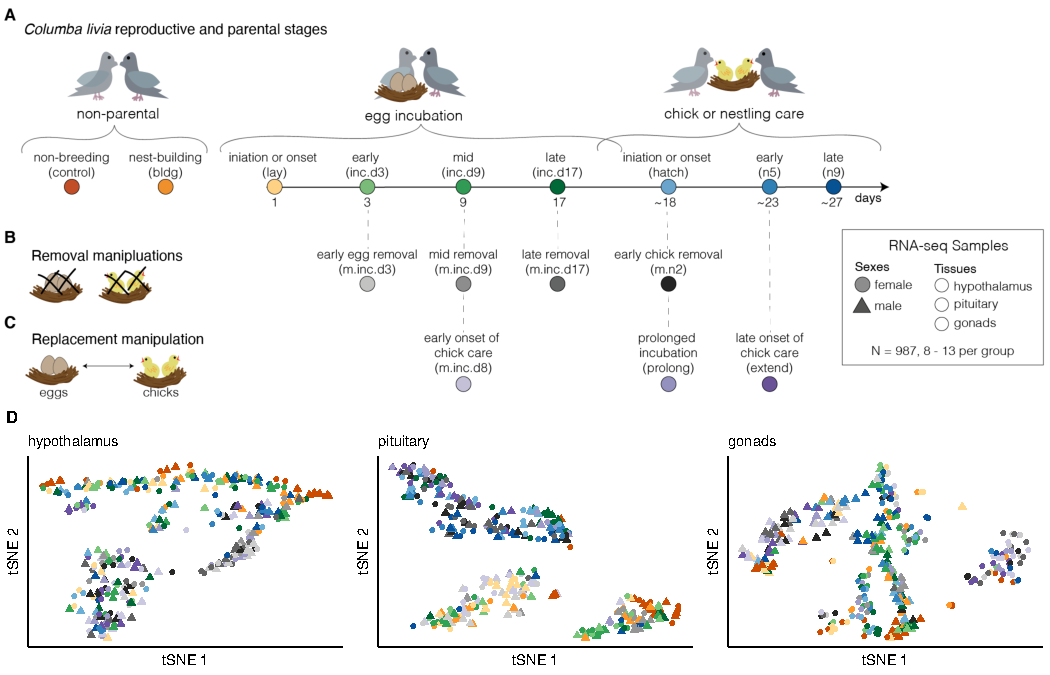
\includegraphics{elife_v1_files/figure-latex/fig1-1} \caption[Experimental design]{Experimental design. A) We investigated nine timepoints that spanned the majority of reproductive efforts in this species. These timepoints consisted of a "control" or non-parenting state (from MacManes et al 2016 and Calisi et al. 2017), nest-building, clutch initiation or the onset of incubation, clutch completion and early incubation, mid-incubation, late incubation, initiation of nestling care, early nestling care, and mid-nestling care. To teste whether external or internal factors were regulating gene activity, we also conducted a series of offspring removal (B) and replacement (C) manipulations to test whether transcriptional changes were dependent upon offspring presence or were regulated by an internal clock. (D) We used t-Distributed Stochastic Neighbor Embedding (t-SNE) to reduce the dimensionality of the transcriptomes from the hypothalamus, pituitary, and gonads of male and female rock. Circles and triangles represent female and male samples, respectively, and points are colored by treatment.}\label{fig:fig1}
\end{figure}
\end{Schunk}

\begin{Schunk}
\begin{figure}
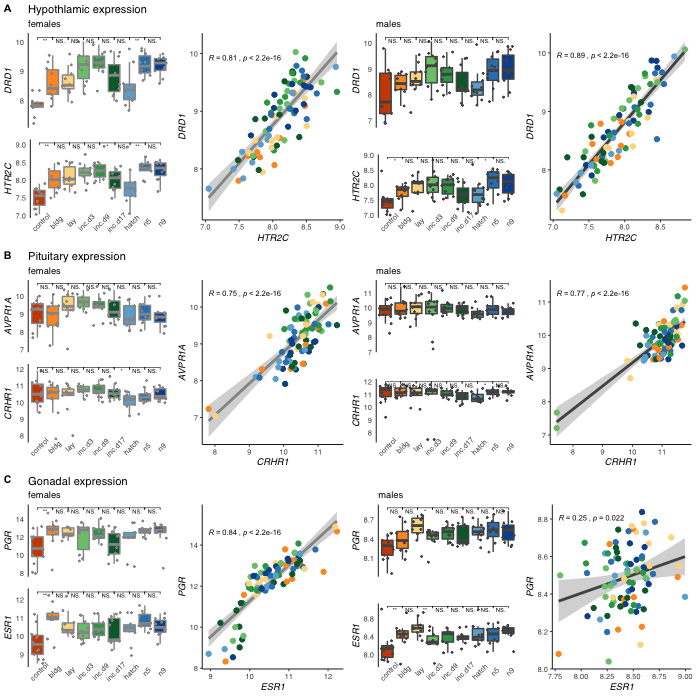
\includegraphics{elife_v1_files/figure-latex/fig2-1} \caption[Hypothesis-driven and data-driven approaches to identifying changes in gene expression.Box-and-whisker plots show changes in gene expression of serotonin receptor (HTR2C) in the hypothalamus (A), prolactin (PRL) in the pituitary (B), and estrogen receptor 1 (ESR1) in the gonads.Bar and statistics are shown for one contrast of interest between treatment groups]{Hypothesis-driven and data-driven approaches to identifying changes in gene expression.Box-and-whisker plots show changes in gene expression of serotonin receptor (HTR2C) in the hypothalamus (A), prolactin (PRL) in the pituitary (B), and estrogen receptor 1 (ESR1) in the gonads.Bar and statistics are shown for one contrast of interest between treatment groups. Boxes are colored by treatment. Volcano plots show the log-fold change (LFC) and -log10(FDR) for all genes that are significantly different differentially between the aforementioned treatment groups. Boxes are colored by the treatment were gene expression was higher.}\label{fig:fig2}
\end{figure}
\end{Schunk}

\begin{Schunk}
\begin{figure}
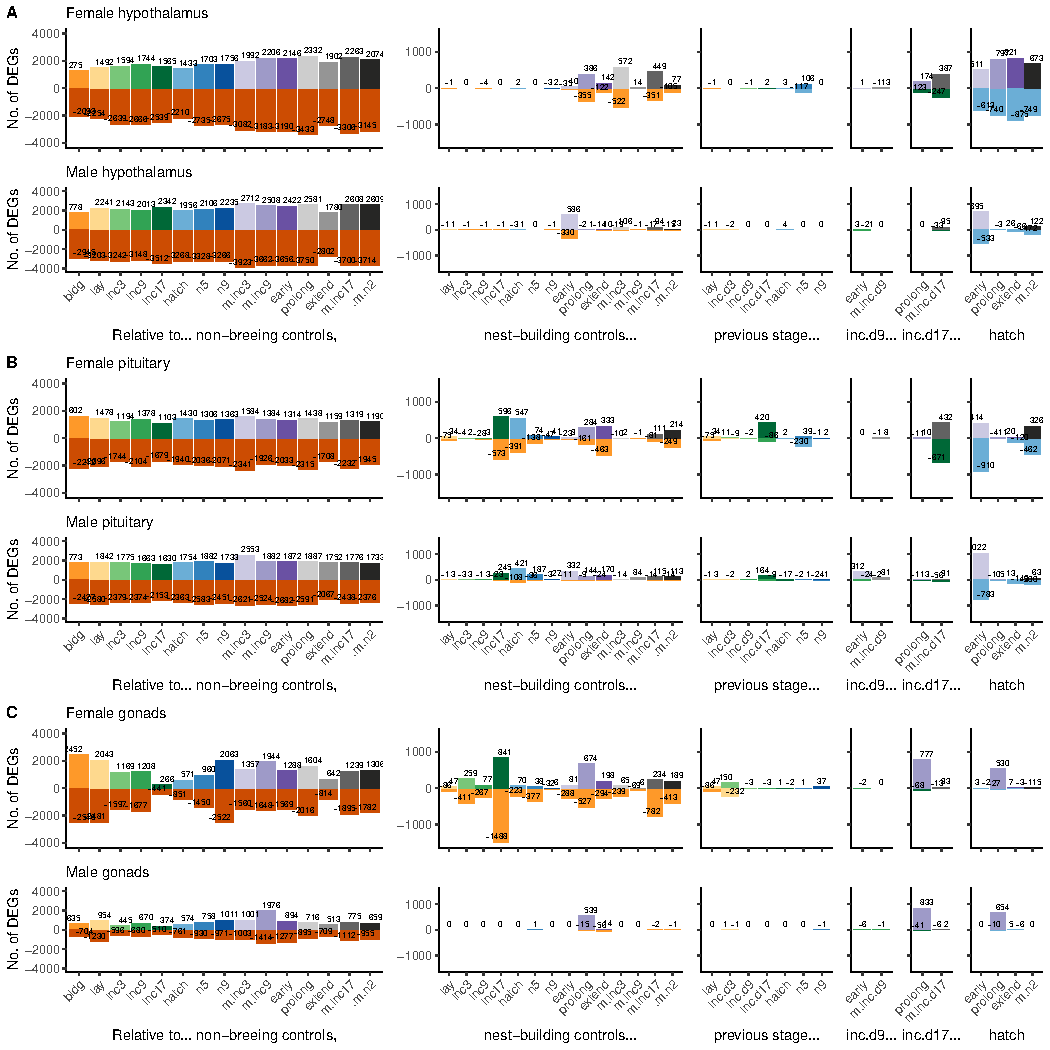
\includegraphics{elife_v1_files/figure-latex/fig3-1} \caption[Summary of differentially expressed genes]{Summary of differentially expressed genes. Bar plots show the total number of significantly differentially expressed genes for all two-way comparisons in the hypothalamus (A), pituitary (B), gonads (C) . Contrasts are made relative to the non-breeding controls, the nest-building group, the previous stage, or the internal or external control group. Bars are colored by the treatment where gene expression was higher. A negative number of differentially expressed genes means that many genes had increase expression in the reference group.}\label{fig:fig3}
\end{figure}
\end{Schunk}

\newpage

\hypertarget{references}{%
\subsection{References}\label{references}}

\bibliography{RJreferences}

\hypertarget{acknowledgements}{%
\subsection{Acknowledgements}\label{acknowledgements}}

Thanks to Owen for discussion of data sonfification. Thanks to DIB lab
members for software and methods discussion (Titus, Taylor, Luiz,
Amanda, Alicia, Picaso). We thank Pacha for help with database and
Shiny. We thank Irene, Erica, Beth Krestoff and Tiffany Chen for
assistance in managing the aviary and collecting nest stage data. We
thank Candice Lee, Annie Bond, and Tanner Feustel and others?? for
assistance with tissue collections. We thank Dr.~Fred Angelier for
performing the prolactin RIA.This research was supported by NSF IOS
1455960 to R.M.C. and M.D.M. Author contributions: RMC designed the
experiment. RMC and MDM acquired funding. SHA contributed to the
experimental design by adding several time points. SHA, with the
assistance of VF, AB, and RMC, conducted the data collection. SHA and a
team of trained undergraduate students biopsy punched the hypothalami
and lateral septum. ASL extracted the RNA, created the libraries, and
conducted all early bioinformatic work. RMH conducted all later analyses
of the genomic data. RMH and SHA drafted the manuscript and all other
authors provided edits.

\hypertarget{author-affiliations}{%
\subsection{Author affiliations}\label{author-affiliations}}


\address{%
Suzanne H. Austin \footnote{equal contribtion, currently at the
  University of Oregon}\\
University of California, Davis\\
\\
}
\href{mailto:suzannehaustin@gmail.com}{\nolinkurl{suzannehaustin@gmail.com}}

\address{%
Rayna M Harris \footnote{equal contribtion}\\
University of California, Davis\\
\\
}


\address{%
Andrew S. Lang\\
University of New Hampshire\\
\\
}


\address{%
Victoria S. Farrar\\
University of California, Davis\\
\\
}


\address{%
April Booth\\
University of California, Davis\\
\\
}


\address{%
Tanner Feustel\\
University of California, Davis\\
\\
}


\address{%
Matthew D. MacManes\\
University of New Hampshire\\
\\
}


\address{%
Rebecca M. Calisi \footnote{corresponding author}\\
University of California, Davis\\
\\
}
\href{mailto:rmcalisi@ucdavis.edu}{\nolinkurl{rmcalisi@ucdavis.edu}}

